% !TeX root = ../presentation.tex

\section[AFRL Work]{Previous Air Force work}
\subsection[ANGELS]{Tracking/Validation of GPS on ANGELS}

\begin{frame}{Global Positioning System}
    \begin{itemize}
        \item GPS satellites orbit at \( \approx \SI{26000}{\kilo\meter} \)
        \item Trilateration - Multiple cooperative transmitters allow for geolocation
    \end{itemize}
    \only<1>{
    \begin{center}
        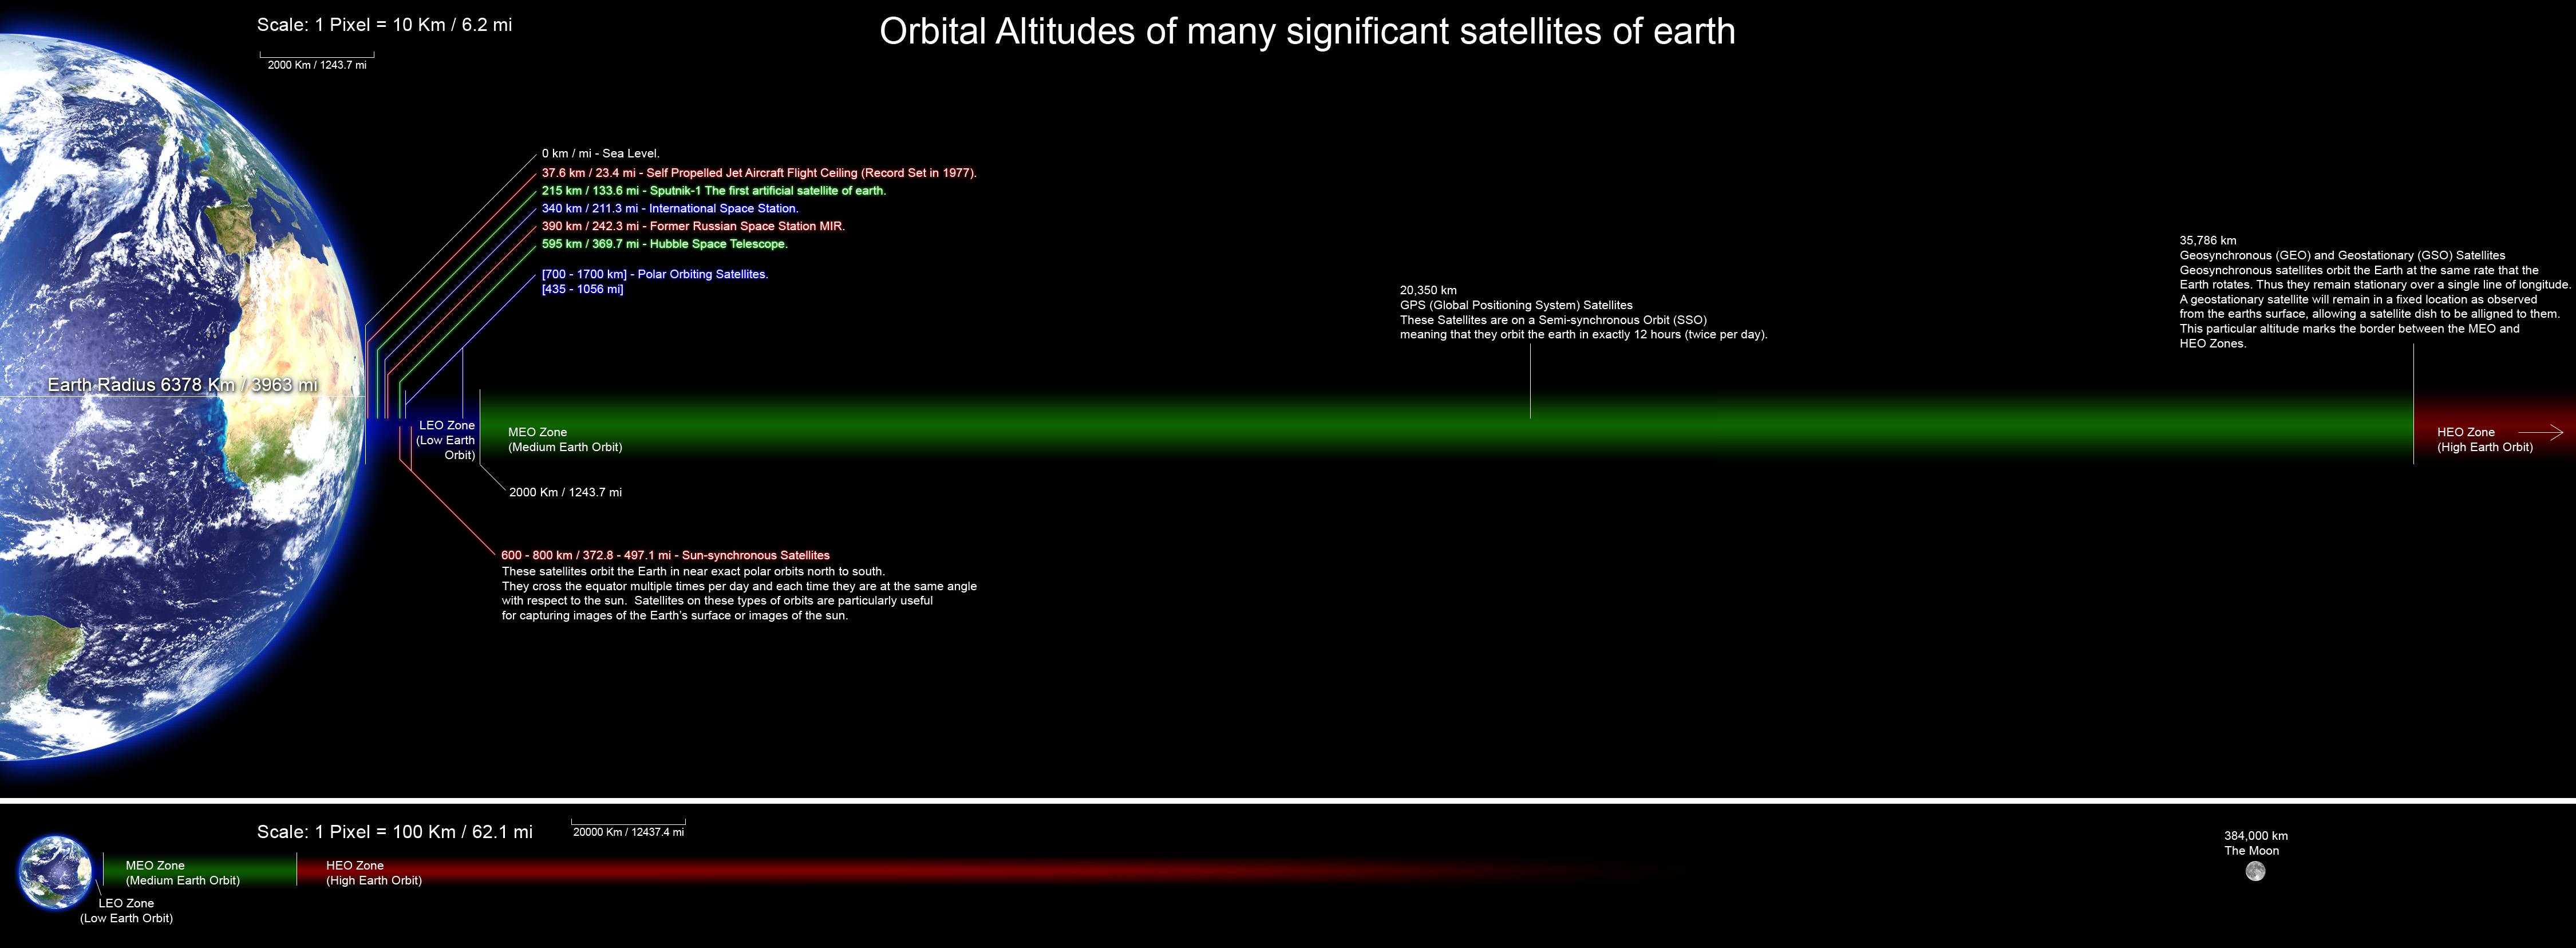
\includegraphics[width=\textwidth,height=0.7\textheight,keepaspectratio]{figures/airforce/Orbitalaltitudes.jpg}
    \end{center}
    }
    \only<2>{
    \begin{center}
        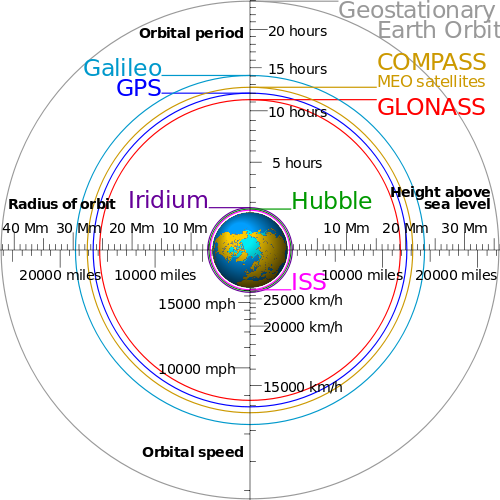
\includegraphics[width=\textwidth,height=0.8\textheight,keepaspectratio]{figures/airforce/geostationary.png}
    \end{center}
    }
\end{frame}

\begin{frame}[t]\frametitle{ANGELS}
    \framesubtitle{Automated Navigation and Guidance Experiment for Local Space}
    \begin{itemize}
        \item Test algorithms/procedures for close proximity operations
        \item Launched in 2014 to a super-geo orbit (less than \SI{24}{\hour} period)
        \item Onboard GPS reciever - accurate positioning outside GPS constellation?
    \end{itemize}
    \begin{center}
        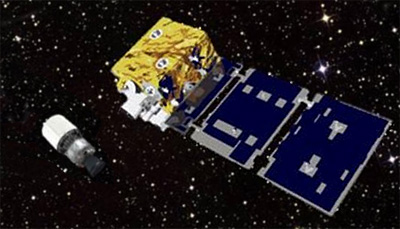
\includegraphics[width=0.5\textwidth,height=0.8\textwidth,keepaspectratio]{figures/airforce/angels.jpg}
    \end{center}
\end{frame}

\begin{frame}[t]\frametitle{Space Survelliance Network}
    \begin{columns}
    \begin{column}{0.5\textwidth}
        \begin{itemize}
            \item<1-> Collection of USAF sensors around the world
            \item<2-> Offers tracking data on \( > 20000  \) objects
            \item<3-> Legacy system with a variety of issues
            \begin{itemize}
                \item Scheduling of collects
                \item Information loss between sensor and catalog
                \item Dynamic modeling
                \item State representation (TLEs)
                \item Uncertainty metrics
            \end{itemize}
        \end{itemize}
    \end{column}
    \begin{column}{0.5\textwidth}
        \begin{center}
            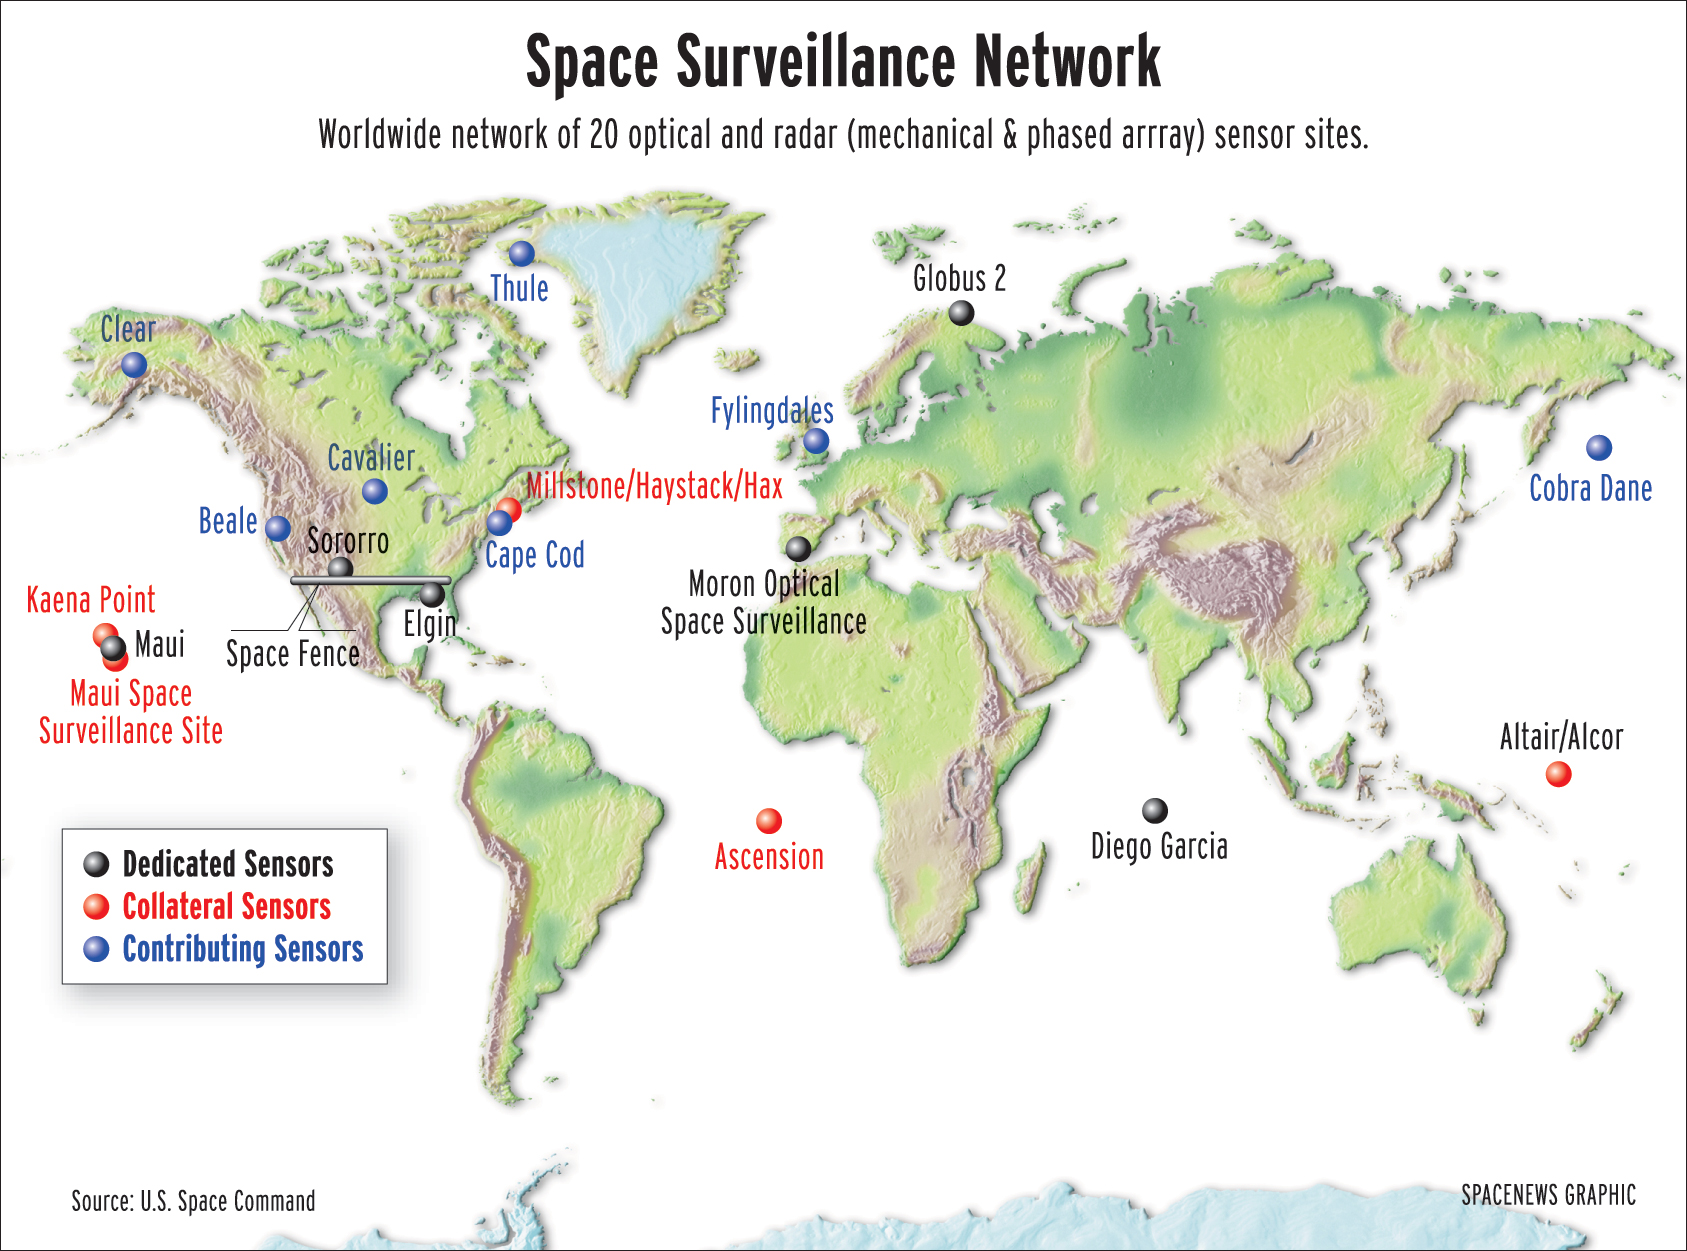
\includegraphics[width=\textwidth,height=0.6\textheight,keepaspectratio]{figures/airforce/ssn.jpg}
        \end{center}
    \end{column}
    \end{columns}
\end{frame}

\begin{frame}[t]{GPS V\&V experiment}
    \framesubtitle{GPS verification and validation}
    \begin{itemize}
        \item<1-> Need accurate state knowledge to operate ``close'' to other spacecraft
        \begin{itemize}
            \item Is GPS even functional at that altitude?
            \item What kind of accuracy is possible?
            \item How do we even know if the GPS solution is ``correct''?
        \end{itemize}
        \item<2-> Independent method of determining ANGELS position
        \begin{itemize}
            \item Ground based observations for orbit determination
            \item Independently estimate state, rather than use JSPOC
            \item Statistically compare GPS vs. Ground OD 
            \item How much data/how fast can we do OD?
            \item Is there a GEO satellite with accurate position?
        \end{itemize}
    \end{itemize}
\end{frame}

\begin{frame}[t]\frametitle{Research Results}
    \begin{columns}
    \begin{column}{0.5\textwidth}
    \begin{itemize}
        \item Asymmetric spacecraft - momentum management is key
        \begin{itemize}
            \item OD requires a non-maneuvering spacecraft
            \item Flipping maneuver enables 2 week quiescent period
        \end{itemize}
        \item OD campaign on operational satellites
        \begin{itemize}
            \item Test campaign on Galaxy 15
        \end{itemize}
    \end{itemize}
    \end{column}
    \begin{column}{0.5\textwidth}
        \begin{center}
            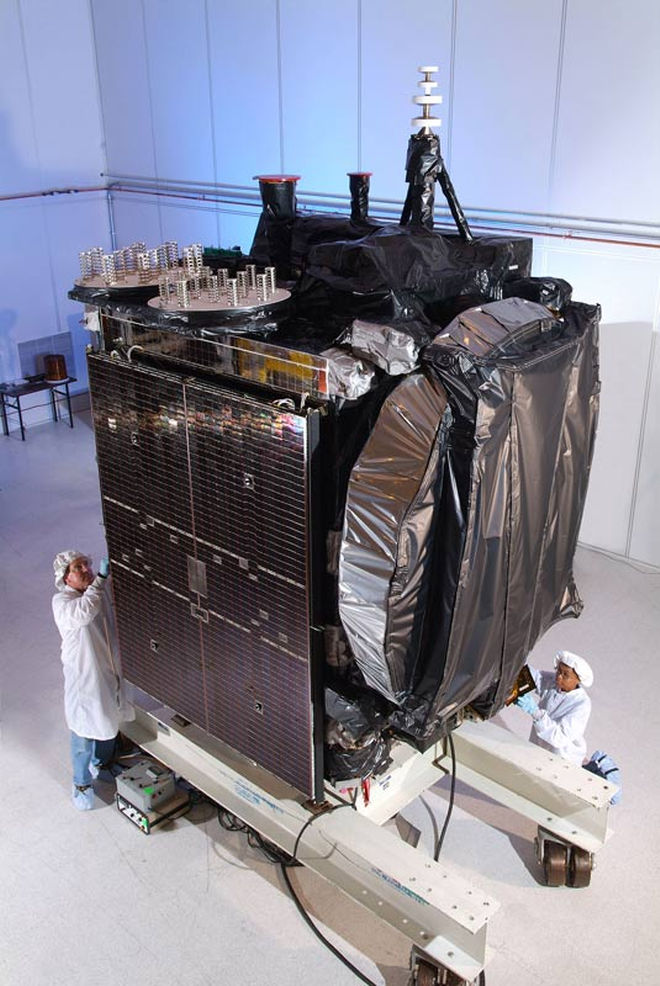
\includegraphics[width=\columnwidth,height=0.6\textheight,keepaspectratio]{figures/airforce/galaxy15.jpg}
        \end{center}
    \end{column}
    \end{columns}
    \begin{block}{OD Results}
        Able to achieve \( \leq \SI{15}{\meter} \) OD solution with 3 days of ``high priority'' SSN measurements on Galaxy 15 WAAS.
    \end{block}
\end{frame}

\subsection[Space TDOA]{Space based geolocation using TDOA}

\begin{frame}[t]\frametitle{Geolocation}
    \begin{itemize}
        \item Variety of possible localization methods
        \begin{itemize}
            \item \Emph{Multilateration} - time/range differences between transmitter and receiver (LORAN-C)
            \item \Emph{Trilateration} - range measurements between transmitter and receiver (GPS)
            \item \Emph{Triangulation} - angular/bearing measurements to known transmitter locations (land navigation)
        \end{itemize}
    \end{itemize}

    \begin{block}{Space Based Time Difference of Arrival Localization}
        Determine the position of a transmitter based on measurements from a constellation of satellites
    \end{block}
\end{frame}

\begin{frame}[t]{TDOA - Time Difference of Arrival}
    \begin{itemize}
        \item The arrival time of a signal at differing reciever stations
        \begin{itemize}
            \item TDOA/RDOA - time difference \( \equiv \) range difference
        \end{itemize}
        \item Locus of possible transmitter positions defines a hyperbola 
        \begin{itemize}
            \item Constant range difference between pairs of stations located at the foci
            \item Given 4 receivers and the surface of the Earth we can uniquely locate the transmitter
            \item Algebraic as well as iterative/recursive based approaches investigated
        \end{itemize}
    \end{itemize}

    \begin{center}
        \only<1>{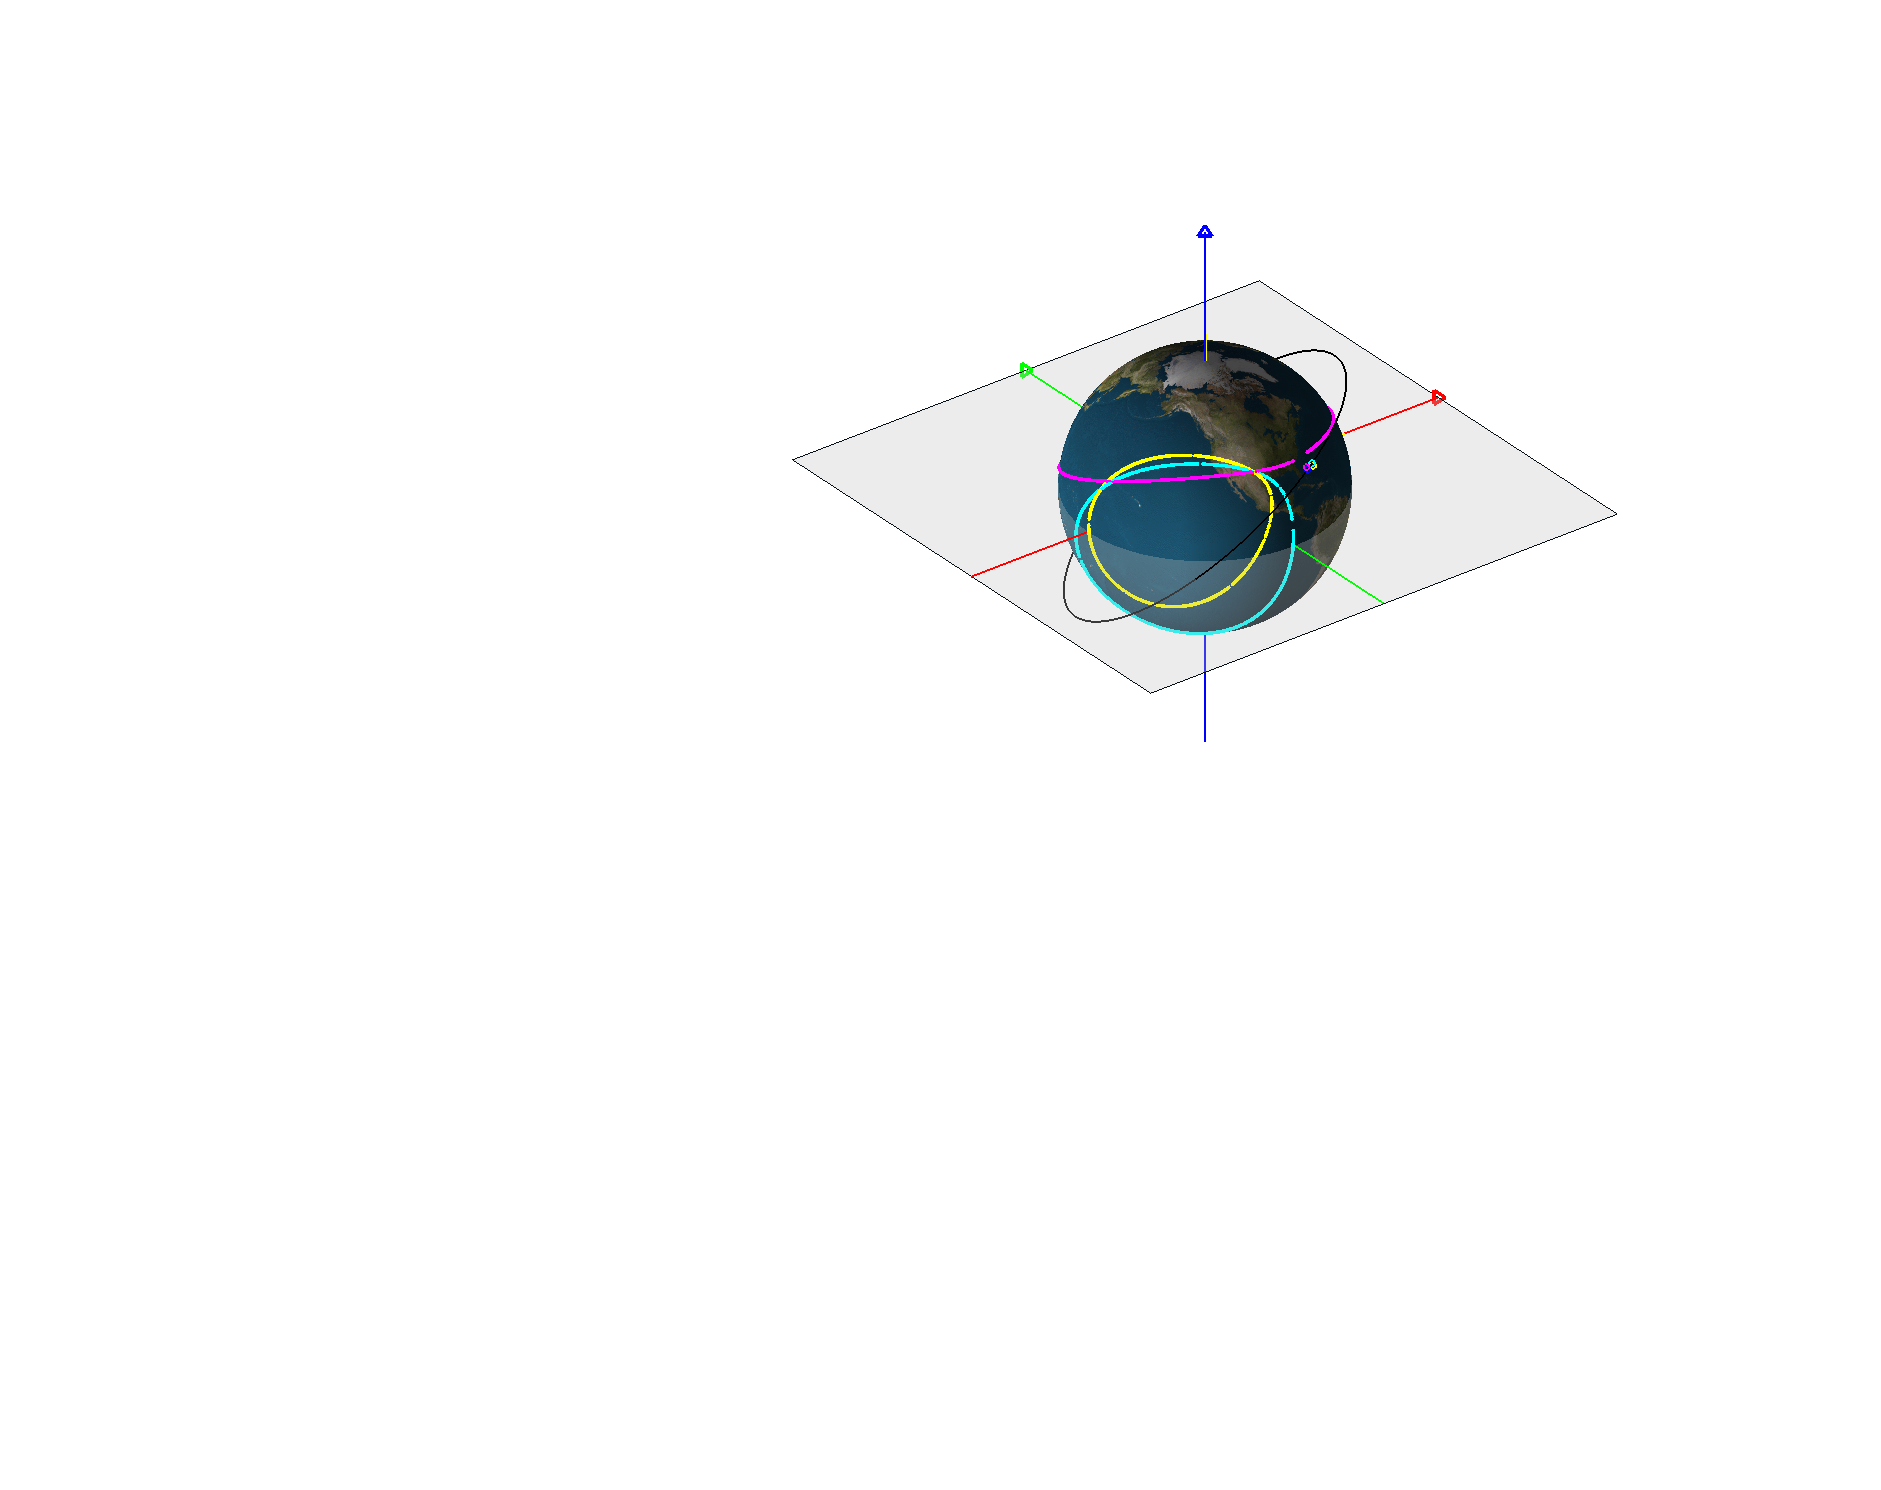
\includegraphics[width=0.5\textwidth,height=0.5\textheight,keepaspectratio]{figures/airforce/tdoa_curves_globe.pdf}~
        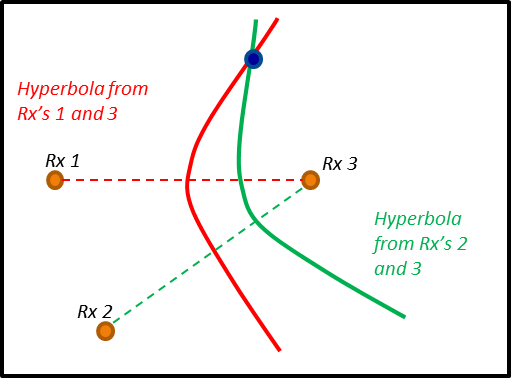
\includegraphics[width=0.5\textwidth,height=0.5\textheight,keepaspectratio]{figures/airforce/hyperbola.png}}
        \only<2>{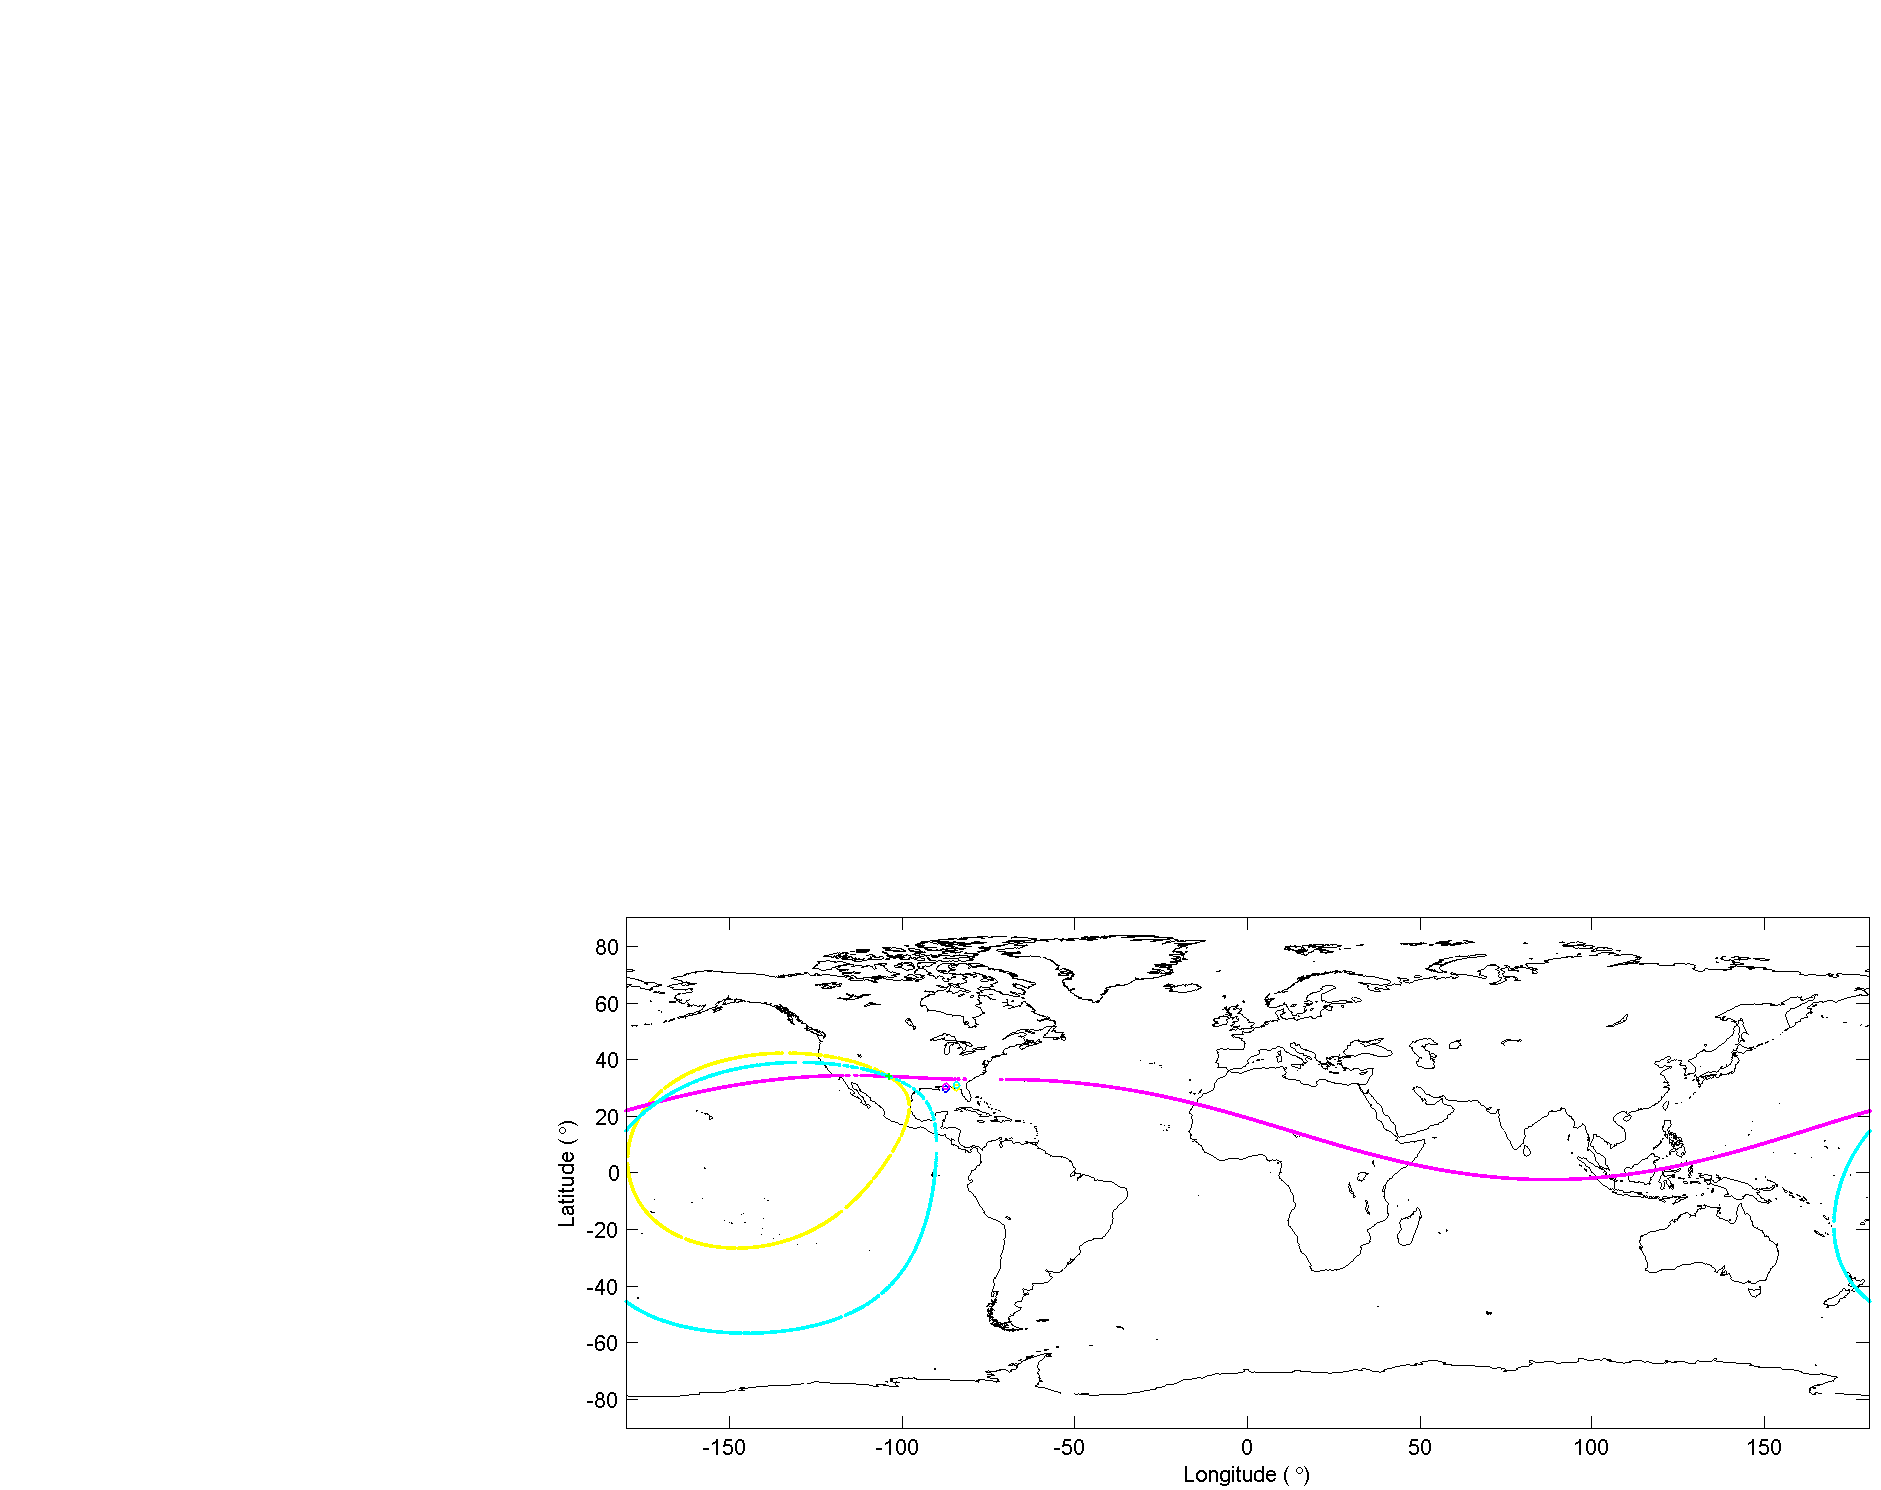
\includegraphics[width=\textwidth,height=0.5\textheight,keepaspectratio]{figures/airforce/tdoa_curves_mercator.pdf}}
    \end{center}
\end{frame}
